\documentclass[conference]{IEEEtran}
\IEEEoverridecommandlockouts

\usepackage{cite}
\usepackage{amsmath,amssymb}
\usepackage{graphicx}
\usepackage{array}
\usepackage{tabularx}
\usepackage{booktabs}
\usepackage{xcolor}
\usepackage[hidelinks]{hyperref}
\urlstyle{same}
\graphicspath{{figures/}}

% ------------------------------------------------------------------
% DRAFT MARKERS: every \tbd{...} is a value or passage still to be
% filled in after the final evaluation. Search for "\tbd" before
% submitting; the final PDF must contain no red text.
% ------------------------------------------------------------------
\newcommand{\tbd}[1]{\textcolor{red}{\textbf{[TBD: #1]}}}

\begin{document}

% ============================================================
% 1. TITLE PAGE
% ============================================================
\title{Comparative Study of Image Classification Robustness Under Visual Degradation\\[2pt]
{\large\itshape Phase II Report: Implementation and Evaluation (Track 2: Comparative Study)}}

\author{%
\textit{Afnan Hashed Ahmed Nasser (223049806), Lulu Abdullah Abdulaziz AlMaghlouth (223036019),}\\
\textit{Batool Hassan Jawad Alawadh (219020376)}\\
College of Computer Sciences \& Information Technology, King Faisal University, Al Ahsa, Saudi Arabia.\\
\textit{Group 2, Section 64 \enspace\textbar\enspace Instructor: Dr. Hala Mohamed Hamdoun \enspace\textbar\enspace Submission Date: November 2026}\\
\textit{GitHub Repository: \url{https://github.com/AfnanNas379/image-classification-robustness}}%
}

\maketitle

\begin{abstract}
We implement and evaluate the comparative study designed in Phase I: a plain CNN (baseline), ResNet-18 and a Vision Transformer (ViT), all trained from scratch on CIFAR-10 with one shared training recipe, so that only the architecture differs. Each model is trained with three random seeds (nine runs) and evaluated on 13 fixed test conditions: the clean test set and Gaussian blur, Gaussian noise, reduced resolution and JPEG compression at three severities each. Robustness is measured by the absolute and relative accuracy drop, corruption error relative to the baseline, the calibrated mean corruption error, and two confidence measures (ECE and ACD). On clean validation data, ResNet-18 reaches \tbd{x}\%, the plain CNN \tbd{x}\% and the ViT \tbd{x}\% (mean over three seeds). \tbd{one or two sentences with the main robustness finding}. The full pipeline, logs and results are released in the project repository and can be reproduced with a single notebook.
\end{abstract}

\begin{IEEEkeywords}
image classification, robustness, visual degradation, CNN, ResNet, Vision Transformer, reproducibility
\end{IEEEkeywords}

% ============================================================
% 2. INTRODUCTION & PROBLEM FORMULATION
% ============================================================
\section{Introduction and Problem Formulation}

\subsection{Refined Problem Statement}
Image classifiers are usually benchmarked on clean images, while deployed systems receive blurred, noisy, low-resolution and compressed inputs~\cite{hendrycks2019}. Published comparisons of CNNs and Transformers under such degradations disagree~\cite{bai2021,wang2023,liu2024}, mainly because architecture is confounded with pretraining data, training recipe and clean accuracy~\cite{erkara2026,liu2024}. Phase I identified five limitations of existing studies (L1--L5) and designed a controlled comparison to address them. Phase II implements that design. The refined problem is: \emph{when a plain CNN, ResNet-18 and a ViT are trained from scratch on the same native low-resolution dataset with an identical recipe, which architecture loses the least accuracy, relative to its own clean accuracy, as blur, noise, resolution loss and JPEG compression become more severe, and does the answer depend on the degradation type?}

\subsection{Task Definition}
\begin{itemize}
\item \textbf{Input:} an RGB image $x \in \{0,\dots,255\}^{32\times32\times3}$, either clean or degraded by an operator $T_{c,s}$ of type $c \in \{\text{blur}, \text{noise}, \text{resolution}, \text{JPEG}\}$ and severity $s \in \{1,2,3\}$.
\item \textbf{Output:} a probability vector $p_m(y\,|\,x)$ over $K = 10$ classes and the predicted label $\hat{y} = \arg\max_y p_m(y\,|\,x)$.
\item \textbf{Task type:} supervised multi-class image classification. Models are trained only on clean images, so the degraded test conditions measure generalization to unseen distribution shifts~\cite{hendrycks2019}.
\end{itemize}

\subsection{Research Questions and Success Criteria}
The study answers four research questions: \textbf{RQ1}, how accuracy changes with severity for each degradation; \textbf{RQ2}, which architecture shows the smallest relative drop once clean accuracy is controlled for; \textbf{RQ3}, whether the ranking depends on the degradation type; and \textbf{RQ4}, which architectural properties best explain the differences. Phase II is considered successful if the following measurable criteria are met:
\begin{enumerate}
\item[\textbf{S1}] \textbf{Complete matrix:} all $3$ models $\times$ $3$ seeds are trained for the full budget and evaluated on all 13 conditions ($9 \times 13 = 117$ evaluations of 10{,}000 images).
\item[\textbf{S2}] \textbf{Adequate training:} every model converges to a clean accuracy in the range expected for its family when trained from scratch on CIFAR-10 (the ViT is expected to trail the CNNs~\cite{dosovitskiy2021,kotyan2024}).
\item[\textbf{S3}] \textbf{Stability:} the standard deviation of clean test accuracy across seeds is at most 1 percentage point (pp) per model, and differences between models are interpreted only when they exceed the seed-to-seed variation.
\item[\textbf{S4}] \textbf{Answered questions:} RQ1--RQ3 are answered with accuracy, absolute drop $\Delta A$ (pp), relative drop RD (\%, primary metric), mCE, CmCE, ECE and ACD, reported as mean $\pm$ standard deviation over three seeds.
\item[\textbf{S5}] \textbf{Reproducibility:} every number in this report can be regenerated from the repository with fixed seeds, and the stored test sets are verified by SHA-256 checksums.
\end{enumerate}

% ============================================================
% 3. PROPOSED METHOD / APPROACH
% ============================================================
\section{Proposed Approach}

\subsection{Candidate Models and Baseline}
Three architectures are compared (Table~\ref{tab:models}). They represent the progression from plain convolution, through residual convolution~\cite{he2016}, to global self-attention~\cite{dosovitskiy2021}. ResNet-18 and the ViT have similar parameter counts (11.2\,M and 12.5\,M), so that differences between them cannot be attributed to model size~\cite{bai2021}. The \textbf{plain CNN is the baseline}: it is the reference model for the corruption error (CE), in the role AlexNet plays in ImageNet-C~\cite{hendrycks2019}. In addition, each model's own clean accuracy is the baseline for its accuracy drop, and chance accuracy ($\alpha = 0.10$) is the lower bound of the calibrated error~\cite{liu2024}. The ViT uses the standard patch embedding without PreLayerNorm, so that the contrast mechanism reported by Kim \emph{et al.}~\cite{kim2023} is not masked.

\begin{table}[!t]
\caption{Candidate Models ($32\times32$ Input, 10 Classes)}
\label{tab:models}
\centering
\footnotesize
\renewcommand{\arraystretch}{1.15}
\begin{tabular}{@{}>{\raggedright\arraybackslash}p{0.14\columnwidth} >{\raggedright\arraybackslash}p{0.41\columnwidth} r >{\raggedright\arraybackslash}p{0.14\columnwidth}@{}}
\toprule
\textbf{Model} & \textbf{Configuration} & \textbf{Params} & \textbf{Role}\\
\midrule
Plain CNN & 6 conv $3\times3$ (64-64-128-128-256-256), BN, ReLU, 2 max-pools, GAP, dropout 0.3 & 1{,}148{,}874 & Baseline, CE reference\\
ResNet-18~\cite{he2016} & CIFAR stem ($3\times3$ conv, no max-pool); 4 stages $\times$ 2 basic blocks (64--512); GAP & 11{,}173{,}962 & Residual CNN\\
ViT~\cite{dosovitskiy2021} & $4\times4$ patches (64 tokens + [CLS]), $D = 384$, 7 pre-norm blocks, 6 heads, MLP 1{,}536, dropout 0.1, learnable positions & 12{,}470{,}026 & Self-attention\\
\bottomrule
\end{tabular}
\end{table}

\subsection{Rationale for the Comparison}
The comparison is designed so that \emph{only the architecture varies}. All three models see the same 45{,}000 training images in the same order for a given seed, use the same optimizer, schedule, augmentation and epoch budget, are selected by the same criterion, and are tested on the same stored degraded images. This addresses L1 (no pretraining, one recipe), L2 (plain CNN, ResNet and ViT in one pipeline), L3 (native $32\times32$ data without upsampling), L4 (RD and CmCE remove the dependence on clean accuracy; ECE and ACD measure confidence) and L5 (four degradation types, including reduced resolution, with severities checked by PSNR and SSIM~\cite{wang2004}). Three seeds per model make it possible to separate architectural effects from training noise.

\subsection{Evaluation Metrics}
For model $m$, degradation $c$ and severity $s$, with $N = 10{,}000$ test images:
\begin{align}
\mathrm{Acc}_{m,c,s} &= \tfrac{1}{N}\textstyle\sum_{i=1}^{N} \mathbf{1}\!\left[\hat{y}_m\big(T_{c,s}(x_i)\big) = y_i\right] \label{eq:acc}\\
\Delta A_{m,c,s} &= \mathrm{Acc}_{m,\mathrm{clean}} - \mathrm{Acc}_{m,c,s} \label{eq:drop}\\
\mathrm{RD}_{m,c,s} &= \Delta A_{m,c,s} / \mathrm{Acc}_{m,\mathrm{clean}} \times 100\% \label{eq:rd}\\
\mathrm{CE}_{m,c} &= \textstyle\sum_{s} E_{m,c,s} \big/ \sum_{s} E_{\mathrm{ref},c,s} \label{eq:ce}\\
\mathrm{CmCE}_m &= \left(1 - \mathrm{m}E_m - \alpha\right) / \left(\mathrm{Acc}_{m,\mathrm{clean}} - \alpha\right) \label{eq:cmce}
\end{align}
where $E = 1 - \mathrm{Acc}$ is the error, the reference model is the plain CNN with the same seed, and $\mathrm{m}E_m$ is the mean error over the 12 degraded conditions. $\Delta A$ is reported in pp and RD in \%; RD is the primary measure. mCE is the mean of \eqref{eq:ce} over the four types (the plain CNN has mCE $= 1$ by definition), and the relative CE uses the error \emph{increase} over the clean error instead of the error itself~\cite{hendrycks2019}. CmCE $= 1$ means no loss and $0$ means chance level~\cite{liu2024}. Confidence is assessed with the Expected Calibration Error (ECE) with 15 equal-width bins~\cite{guo2017} and the Accuracy--Confidence Divergence $D_c = \frac{1}{3}\sum_s(\mathrm{Acc}_{c,s} - \overline{\mathrm{Conf}}_{c,s})$, where a negative value means overconfidence, together with $N_c$, the number of severities whose gap has the same sign as $D_c$~\cite{erkara2026}. All metrics are computed per seed and reported as mean $\pm$ standard deviation over the three seeds.

% ============================================================
% 4. SYSTEM DESIGN & ARCHITECTURE
% ============================================================
\section{System Design and Architecture}

\begin{figure*}[!t]
\centering
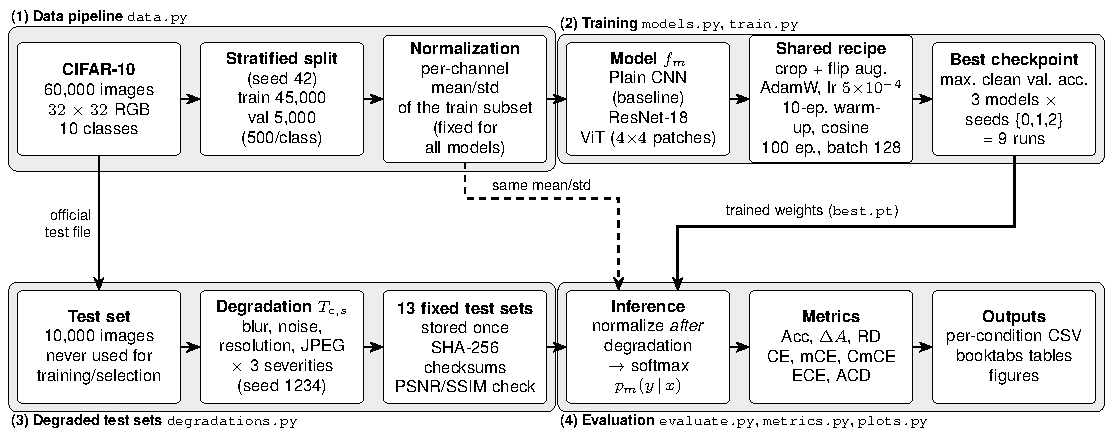
\includegraphics[width=\textwidth]{architecture.pdf}
\caption{System architecture. (1) The data pipeline creates the fixed split and the normalization statistics. (2) Each model is trained with the shared recipe and the checkpoint with the best clean validation accuracy is kept. (3) The 13 test sets are generated once and stored with checksums. (4) Every trained model is evaluated on the same stored images, normalized with the same statistics, and the metrics, tables and figures are produced automatically. Repository modules are shown next to each stage.}
\label{fig:arch}
\end{figure*}

Fig.~\ref{fig:arch} shows the data $\rightarrow$ model $\rightarrow$ output pipeline. It consists of four stages, each implemented as a separate module in \texttt{src/}, with one shared configuration file (\texttt{configs/default.yaml}) that holds every setting. Images remain 8-bit integer arrays until the final step, so training and test images, clean or degraded, pass through exactly the same conversion and normalization.

\subsection{Workflow}
The complete experiment is run by the notebook \texttt{notebooks/colab\_run.ipynb}, which calls the following steps:
\begin{enumerate}
\item \textbf{Setup.} Clone the repository, install the pinned requirements and link \texttt{data/}, \texttt{runs/} and \texttt{results/} to persistent storage.
\item \textbf{Data and test sets.} The script \texttt{scripts/make\_degraded.py} downloads CIFAR-10, creates the stratified train/validation split (seed 42), verifies it (no overlap, no missing images, 500 validation images per class), applies the 13 conditions to the 10{,}000 test images (seed 1234), and stores each condition with its SHA-256 checksum and mean PSNR and SSIM in a manifest.
\item \textbf{Training} (\texttt{python -m src.train --model $m$ --seed $k$}). Train one model with one seed for 100 epochs. After every epoch the script appends a row to \texttt{log.csv}, saves the best checkpoint (\texttt{best.pt}) and a full resume checkpoint (\texttt{last.pt}) with model, optimizer, scaler and random-number-generator states. A finished run is marked by \texttt{done.json}; \texttt{meta.json} records the configuration, split check, normalization statistics, software version and GPU.
\item \textbf{Evaluation} (\texttt{python -m src.evaluate}). Load each finished \texttt{best.pt}, predict all 13 stored test sets, and save per-condition accuracy, mean confidence, ECE and NLL, the predictions of every image, the summary metrics of Section~II-C, and the booktabs \LaTeX\ tables used in this report.
\item \textbf{Figures} (\texttt{python -m src.plots}). Generate accuracy and ECE versus severity, RD per degradation type, training curves and degradation examples, as PDF and 300-dpi PNG with markers and line styles that remain distinguishable in greyscale.
\item \textbf{Export.} Collect the CSV files, tables, figures, logs and manifest for the repository. Checkpoints and image arrays are not committed because of their size; they are regenerated deterministically by steps 2 and 3.
\end{enumerate}

% ============================================================
% 5. DATASET DESCRIPTION
% ============================================================
\section{Dataset Description}

\subsection{CIFAR-10}
CIFAR-10~\cite{krizhevsky2009} (\url{https://www.cs.toronto.edu/~kriz/cifar.html}, loaded with \texttt{torchvision.datasets.CIFAR10}) contains 60{,}000 RGB images of $32\times32$ pixels in 10 balanced classes (airplane, automobile, bird, cat, deer, dog, frog, horse, ship, truck): 50{,}000 training images (5{,}000 per class) and 10{,}000 test images (1{,}000 per class).

\subsection{Split}
From the 50{,}000 training images, 500 per class are drawn at random (seed 42) as a stratified validation set of 5{,}000 images, leaving 45{,}000 for training (4{,}500 per class). The split is checked by code before every run: train and validation do not overlap, together they contain all 50{,}000 images, and every class has exactly 500 validation images. The validation set is used only to select the best epoch; the 10{,}000 test images are used only for the final evaluation and never for training or model selection.

\subsection{Preprocessing}
\begin{enumerate}
\item \textbf{Normalization:} each channel is standardized with the mean $(0.4918, 0.4825, 0.4468)$ and standard deviation $(0.2471, 0.2435, 0.2617)$ of the 45{,}000 training images only, so no validation or test information leaks into training. The same statistics are used for every model and are applied \emph{after} degradation, as a deployed system would do.
\item \textbf{Training augmentation:} random $32\times32$ crop after 4-pixel zero padding and random horizontal flip, both drawn from the seeded generator of the run.
\item \textbf{No resizing:} all models work at the native $32\times32$ resolution (addressing L3).
\end{enumerate}

\subsection{Degraded Test Sets}
The four degradations of Table~\ref{tab:degradations} are applied to the 10{,}000 test images. Blur uses a Gaussian kernel with reflect padding; noise is added on the $[0,1]$ scale with a fixed seed per level and clipped; reduced resolution downsamples to $r\times r$ and upsamples back to $32\times32$ with bicubic interpolation; JPEG encodes and decodes with 4:2:0 chroma subsampling. Each set is rounded to 8-bit integers, stored once and loaded by every model, so all models are evaluated on identical pixels. As planned in Phase I, the mean PSNR and SSIM~\cite{wang2004} of each condition against the clean images (Table~\ref{tab:degradations}) are used to compare severities across types.

\begin{table}[!t]
\caption{Degradation Conditions and Measured Distortion (Mean over 10{,}000 Test Images)}
\label{tab:degradations}
\centering
\footnotesize
\renewcommand{\arraystretch}{1.1}
\setlength{\tabcolsep}{4pt}
\begin{tabular}{@{}llcc@{}}
\toprule
\textbf{Condition} & \textbf{Parameter} & \textbf{PSNR (dB)} & \textbf{SSIM} \\
\midrule
Blur 1 & $\sigma = 0.5$, kernel $5\times5$ & 34.76 & 0.986 \\
Blur 2 & $\sigma = 1.0$, kernel $7\times7$ & 25.44 & 0.866 \\
Blur 3 & $\sigma = 1.5$, kernel $11\times11$ & 22.60 & 0.736 \\
\midrule
Noise 1 & $\sigma_n = 0.04$ & 28.09 & 0.891 \\
Noise 2 & $\sigma_n = 0.08$ & 22.19 & 0.740 \\
Noise 3 & $\sigma_n = 0.12$ & 18.82 & 0.612 \\
\midrule
Resolution 1 & $32\to24\to32$ px & 31.13 & 0.963 \\
Resolution 2 & $32\to16\to32$ px & 26.08 & 0.882 \\
Resolution 3 & $32\to8\to32$ px & 21.14 & 0.633 \\
\midrule
JPEG 1 & quality $Q = 60$ & 29.02 & 0.930 \\
JPEG 2 & quality $Q = 30$ & 26.82 & 0.894 \\
JPEG 3 & quality $Q = 10$ & 23.34 & 0.801 \\
\bottomrule
\end{tabular}
\end{table}

PSNR and SSIM rank the severities consistently. Within every type, distortion increases monotonically with the level, so comparisons of severity levels within a type are valid. Across types, however, equal level numbers do not mean equal distortion: at level~3, Gaussian noise is the harshest condition (18.82\,dB, SSIM 0.612), followed by reduced resolution (21.14\,dB, 0.633) and blur (22.60\,dB, 0.736), while JPEG is the mildest (23.34\,dB, 0.801). At level~1, blur is by far the mildest condition (34.76\,dB, 0.986) and noise again the strongest (28.09\,dB, 0.891). The JPEG levels are also closer together than those of the other types. Differences between degradation types must therefore be interpreted together with these distortion values rather than by level number alone.

% ============================================================
% 6. EXPERIMENTAL SETUP
% ============================================================
\section{Experimental Setup}

\subsection{Tools and Frameworks}
Python 3 with PyTorch 2.11 (CUDA 13.0)~\cite{paszke2019} and torchvision for models and data, NumPy for arrays, Pillow for resizing and JPEG coding, scikit-image for PSNR and SSIM, pandas for result tables, and Matplotlib for figures. All experiments were run on Google Colab; the code also runs locally with \texttt{pip install -r requirements.txt}.

\subsection{Hyperparameters}
All models use the single recipe of Table~\ref{tab:hparams}. The learning rate follows a linear warm-up followed by cosine decay~\cite{loshchilov2017}, updated every step, and AdamW~\cite{loshchilov2019} applies weight decay to weights only (not to biases, normalization parameters, positional embedding or [CLS] token). Mixed precision~\cite{micikevicius2018} is used on the GPU, and gradients are clipped to norm 1.0. The checkpoint with the highest clean validation accuracy is kept for testing. No hyperparameter was tuned on the test set.

\begin{table}[!t]
\caption{Shared Training Recipe (Identical for All Models)}
\label{tab:hparams}
\centering
\footnotesize
\renewcommand{\arraystretch}{1.1}
\begin{tabular}{@{}ll@{}}
\toprule
\textbf{Setting} & \textbf{Value} \\
\midrule
Optimizer & AdamW, $\beta = (0.9, 0.999)$, weight decay 0.05 \\
Peak / final learning rate & $5\times10^{-4}$ / $1\times10^{-6}$ \\
Schedule & 10-epoch linear warm-up, then cosine \\
Epochs / batch size & 100 / 128 (352 steps per epoch) \\
Loss & cross-entropy (no label smoothing) \\
Augmentation & random crop (pad 4) + horizontal flip \\
Regularization & dropout (CNN 0.3, ViT 0.1), gradient clip 1.0 \\
Precision & mixed (FP16 autocast, dynamic loss scaling) \\
Model selection & best clean validation accuracy \\
\bottomrule
\end{tabular}
\end{table}

\subsection{Random Seeds and Determinism}
Three seeds are fixed independently: the data split (seed 42), the degraded test sets (seed 1234) and model training (seeds 0, 1 and 2 for every model). The training seed sets Python, NumPy and PyTorch generators and a dedicated generator for shuffling and augmentation, and cuDNN is set to deterministic mode. Because a resume checkpoint stores all generator states, an interrupted run continues with the same sequence of batches and augmentations; this is verified by an automated test (\texttt{tests/resume\_check.py}) in which an interrupted run and an uninterrupted run end with identical weights.

\subsection{Hardware}
Training and evaluation ran on an NVIDIA Tesla T4 GPU (16\,GB) in Google Colab, as recorded in each run's \texttt{meta.json}. The mean time per epoch was 5.9\,s for the plain CNN, 19.7\,s for ResNet-18 and 33.8\,s for the ViT, i.e.\ about 10, 33 and 56 minutes per 100-epoch run. The nine runs were split across the three team members' Colab accounts by seed.

% ============================================================
% 7. IMPLEMENTATION DETAILS
% ============================================================
\section{Implementation Details}

\subsection{Model Construction}
All models are implemented in PyTorch in \texttt{src/models.py} and checked by parameter count against Table~\ref{tab:models}. The plain CNN stacks three pairs of $3\times3$ convolution--batch-norm--ReLU layers with max-pooling after the first two pairs, followed by global average pooling, dropout and a linear classifier. ResNet-18 follows He \emph{et al.}~\cite{he2016} with the usual CIFAR stem: a $3\times3$ stride-1 first convolution and no initial max-pooling, so that the $32\times32$ input is not reduced too early; residual blocks with a change of stride or width use a $1\times1$ convolutional shortcut. The ViT splits the image into 64 non-overlapping $4\times4$ patches with a strided convolution (equivalent to a linear patch projection), prepends a learnable [CLS] token, adds a learnable positional embedding, and applies seven pre-norm Transformer blocks (multi-head self-attention and a GELU MLP with residual connections); the classifier reads the normalized [CLS] token. Linear layers and embeddings are initialized from a truncated normal distribution ($\sigma = 0.02$).

\subsection{Training and Testing}
The full training split is placed on the GPU as 8-bit tensors; each epoch draws a seeded permutation, augments each batch on the GPU, normalizes it and performs one AdamW step with the scheduled learning rate. After each epoch, validation loss and accuracy are computed on the 5{,}000 validation images. Testing is done only after training, with the selected \texttt{best.pt}: each stored test set is normalized with the training statistics and passed through the model in evaluation mode (dropout off, batch-norm in inference mode), and the softmax outputs are used for accuracy, confidence and calibration. Every metric is computed per seed, and the three seeds are then aggregated.

\subsection{Verification}
Two automated checks run on a CPU without downloading data: a smoke test that executes the whole pipeline (split check, test-set generation, training, evaluation, metrics, tables and figures) on synthetic images, and the resume check described in Section~VI-C. Before evaluation, each run folder was checked to contain exactly one \texttt{best.pt}, \texttt{done.json}, \texttt{log.csv} and \texttt{meta.json}, with 100 consecutive epochs in the log and a best epoch matching \texttt{done.json}.

\subsection{Challenges and Fixes}
\textbf{ViT training instability.} With the first recipe (peak learning rate $10^{-3}$, 5-epoch warm-up), the ViT's validation accuracy collapsed to about 42--45\% during training and reached only 57\% after 100 epochs, while the CNNs trained normally. Because a recipe change for one model would break the fairness of the comparison, the shared recipe was changed for \emph{all} models to a peak learning rate of $5\times10^{-4}$ with a 10-epoch warm-up, and all runs were repeated from scratch. With the new recipe the ViT trained smoothly. The discarded first-recipe runs are archived separately and are not used in any result.

\textbf{Resuming after disconnects.} Colab sessions were interrupted by disconnects and GPU-time limits, so training had to resume from \texttt{last.pt}. The first resume attempt failed with ``RNG state must be a torch.ByteTensor'' because the checkpoint, including the generator states, was loaded directly onto the GPU. The fix loads the checkpoint on the CPU and also saves and restores the CUDA generator state. One run (ViT, seed 0) resumed from a checkpoint created before this fix, without the CUDA generator state; it used the same recipe and data order, but its continuation is not bit-identical to an uninterrupted run.

\textbf{Notebook re-execution.} Re-running the setup cell deleted the folder the notebook was working in, which caused ``Unable to read current working directory''. The cell now changes to \texttt{/content} before re-cloning the repository.

\textbf{Shared-storage duplicates.} The runs were written to one shared Google Drive folder from different accounts. For files written from a collaborator's account rather than the folder owner's, Drive created a new copy at every save instead of replacing the file (e.g., 223 extra files for ResNet-18, seed 0: one log fragment per epoch and one checkpoint per save). No data were lost: the training log was rebuilt from the fragments (100 distinct epochs, no gaps and no conflicting rows), and the final model was identified from the epoch and validation accuracy stored inside each checkpoint, which matched \texttt{done.json} (epoch 89, 94.30\% for ResNet-18; epoch 90, 85.62\% for the ViT). The redundant copies were moved to an archive folder. Afterwards, each member trained into their own storage and the finished runs were collected by one member.

\subsection{Team Contributions}
Afnan implemented the data pipeline and degraded test sets (\texttt{data.py}, \texttt{degradations.py}, \texttt{make\_degraded.py}) and the notebook; Lulu implemented the models and training (\texttt{models.py}, \texttt{train.py}); Batool implemented evaluation, metrics and figures (\texttt{evaluate.py}, \texttt{metrics.py}, \texttt{plots.py}). Each member trained one seed of all three models. The commit history of the repository shows each member's contribution.

% ============================================================
% 8. RESULTS
% ============================================================
\section{Results}

\subsection{Training}
Table~\ref{tab:train} reports the best clean validation accuracy of every run. The seeds of each model agree within \tbd{0.5} pp, and the ranking ResNet-18 $>$ plain CNN $>$ ViT is the same for every seed. Training curves are shown in Fig.~\tbd{training\_curves}.

\begin{table}[!t]
\caption{Best Clean Validation Accuracy (\%) and Epoch per Run}
\label{tab:train}
\centering
\footnotesize
\renewcommand{\arraystretch}{1.1}
\begin{tabular}{@{}lcccc@{}}
\toprule
\textbf{Model} & \textbf{Seed 0} & \textbf{Seed 1} & \textbf{Seed 2} & \textbf{Mean $\pm$ std} \\
\midrule
Plain CNN & 92.12 (93) & 91.96 (87) & \tbd{} & \tbd{} \\
ResNet-18 & 94.30 (89) & 94.10 (92) & \tbd{} & \tbd{} \\
ViT       & 85.62 (90) & 85.14 (98) & \tbd{} & \tbd{} \\
\bottomrule
\end{tabular}
\end{table}

\subsection{Robustness}
\tbd{insert the overall results table generated in results/tables.tex (clean accuracy, $\Delta A$, RD, mCE, CmCE, ECE; mean $\pm$ std over 3 seeds), the RD-per-type table, and the figures accuracy\_vs\_severity, rd\_per\_type and ece\_vs\_severity from results/figures/. Describe for each figure what it shows, with the key numbers, answering RQ1 (severity), RQ2 (overall ranking by RD and CmCE) and RQ3 (ranking per degradation type).}

% ============================================================
% 9. DISCUSSION
% ============================================================
\section{Discussion}
\tbd{to be written after the final evaluation. Planned points: (1) interpretation of the ranking and whether differences exceed seed variation; (2) why each architecture behaves as it does per degradation type (RQ4): local convolution and pooling vs.\ global attention on $4\times4$ patches, frequency content of each degradation, patch-embedding sensitivity~\cite{kim2023,liu2024}; (3) confidence behavior: accuracy falls much faster than confidence under strong degradation (overconfidence, ECE and ACD)~\cite{erkara2026,guo2017}; (4) the effect of unequal severity across types (Table~\ref{tab:degradations}).}

\textbf{Limitations.} \tbd{finalize}: a single dataset at $32\times32$ resolution; three architectures of one size each; one training recipe, chosen to keep the ViT stable rather than tuned per model; only three seeds; synthetic degradations at three severities; severities matched by parameters, not by equal PSNR or SSIM; and one ViT run resumed without the CUDA generator state.

% ============================================================
% 10. CONCLUSION & FUTURE WORK
% ============================================================
\section{Conclusion and Future Work}
Phase II implemented the controlled comparison designed in Phase I as a reproducible pipeline: a verified data split, 13 stored and checksummed test conditions, three models trained from scratch with one shared recipe and three seeds each, and an automated evaluation that produces every table and figure in this report. \tbd{summary of the main findings for RQ1--RQ4}. \tbd{honest statement of anything incomplete}. Future work includes \tbd{e.g., adding PreLayerNorm to the ViT to test the mechanism of Kim \emph{et al.}~\cite{kim2023}; robustness-oriented augmentation applied equally to all models~\cite{nam2024}; more seeds; CIFAR-10-C and larger or higher-resolution datasets; matching severities by measured distortion}.

% ============================================================
% 11. REFERENCES
% ============================================================
\bibliographystyle{IEEEtran}
\bibliography{references}

\end{document}
